A \pythia based study investigating the contributions to the underlying event was undertaken to better understand from a model perspective how the anti-correlation between leading jet $p_{T}$ and transverse region $\langle \Sigma E_{T} \rangle$.
This study was also useful in checking if there was some kind of selection bias arising from ISR/FSR effects causing the anti-correlation.
A sample of 2M \pythia events with a filter requirement of 20 GeV were produced without any UE contributions, with only ISR, with only FSR and with only MPI for comparison to the full \pythia result. 
The UE contributions were turned on/off via commands \texttt{PartonLevel:ISR}, \texttt{PartonLevel:FSR} and \texttt{PartonLevel:MPI}.
The same truth event selection used in the analysis is used in this study.
The MPI contribution is the largest contribution to the UE at RHIC energies across the full jet $p_{T}$ range studied and is also where the anti-correlation between the UE and hard scattering is modeled at least within \pythia.
The FSR/ISR contributions are subdominant to the MPI contribution and are independent of leading jet $p_{T}$ indicating that at least in the modeling of UE at RHIC energies this correlation is not only the result of a selection bias from radiation effects.

\begin{figure}
    \centering
    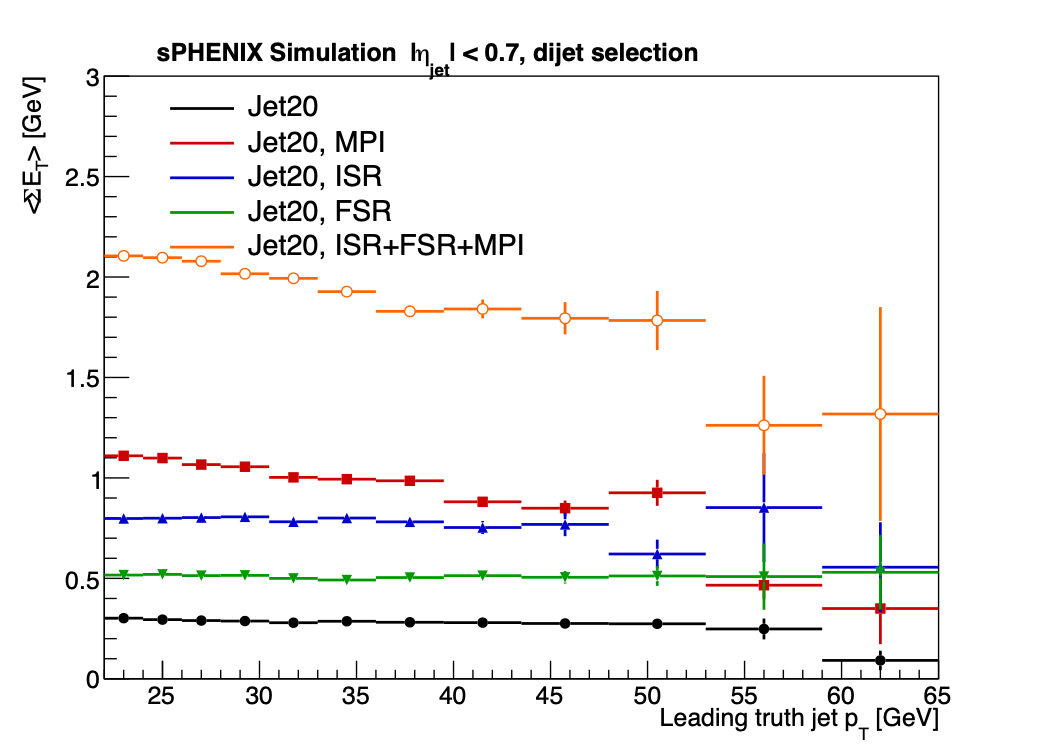
\includegraphics[width=0.7\linewidth]{figures/chapter5/pythia_ue_vs_Pt.png}
    \caption{Average total energy in the transverse region of dijet events as a function of leading jet $p_{T}$ studied in \pythia simulation. Events generated with no ISR/FSR/MPI (black) are compared to events with only MPI (red), only ISR (blue), only FSR (green) and all three UE components (orange).}
    \label{fig:pythia_ue_vs_pt}
\end{figure}